%!TEX root = ../main.tex

\graphicspath{{./figures/chapter2/}}


\chapter{Single RNA Detection}
\label{ch:chapter2}

\minitoc
\newpage


In smFISH images, RNA molecules appear as diffraction limited spots, and for this reason, the detection of individual RNA molecules boils down to spot detection, a problem that has been largely addressed by different scientific communities. 

After a review of different techniques for spot detection, I will discuss shortcomings of existing methods when applied to High Content Screening by \ac{FISH} and describe the solution I have developed and implemented in \mbox{\emph{bigfish.detection}}.
%We try to answer specific limitations of existing solutions, especially the possibility to scale the detection.
%As an example, I also add a code snippet at the end of each step.
Finally I evaluate robustness and accuracy of this implementation by applying the algorithm on simulated data under different noise conditions.

\section{Spot detection as a signal processing problem}
\label{sec:detection_introduction}

This introductory section is devoted to a description of the spot detection problem, and a review of solution proposed in the literature.  

% We first describe inputs and outputs we can expect when we perform spot detection.
% Then we review some solutions proposed in the literature, in bio-informatics, but more generally in computer vision.
% Lastly, we briefly discuss recent methods based on a deep-learning framework.

\begin{figure}[h]
    \centering
    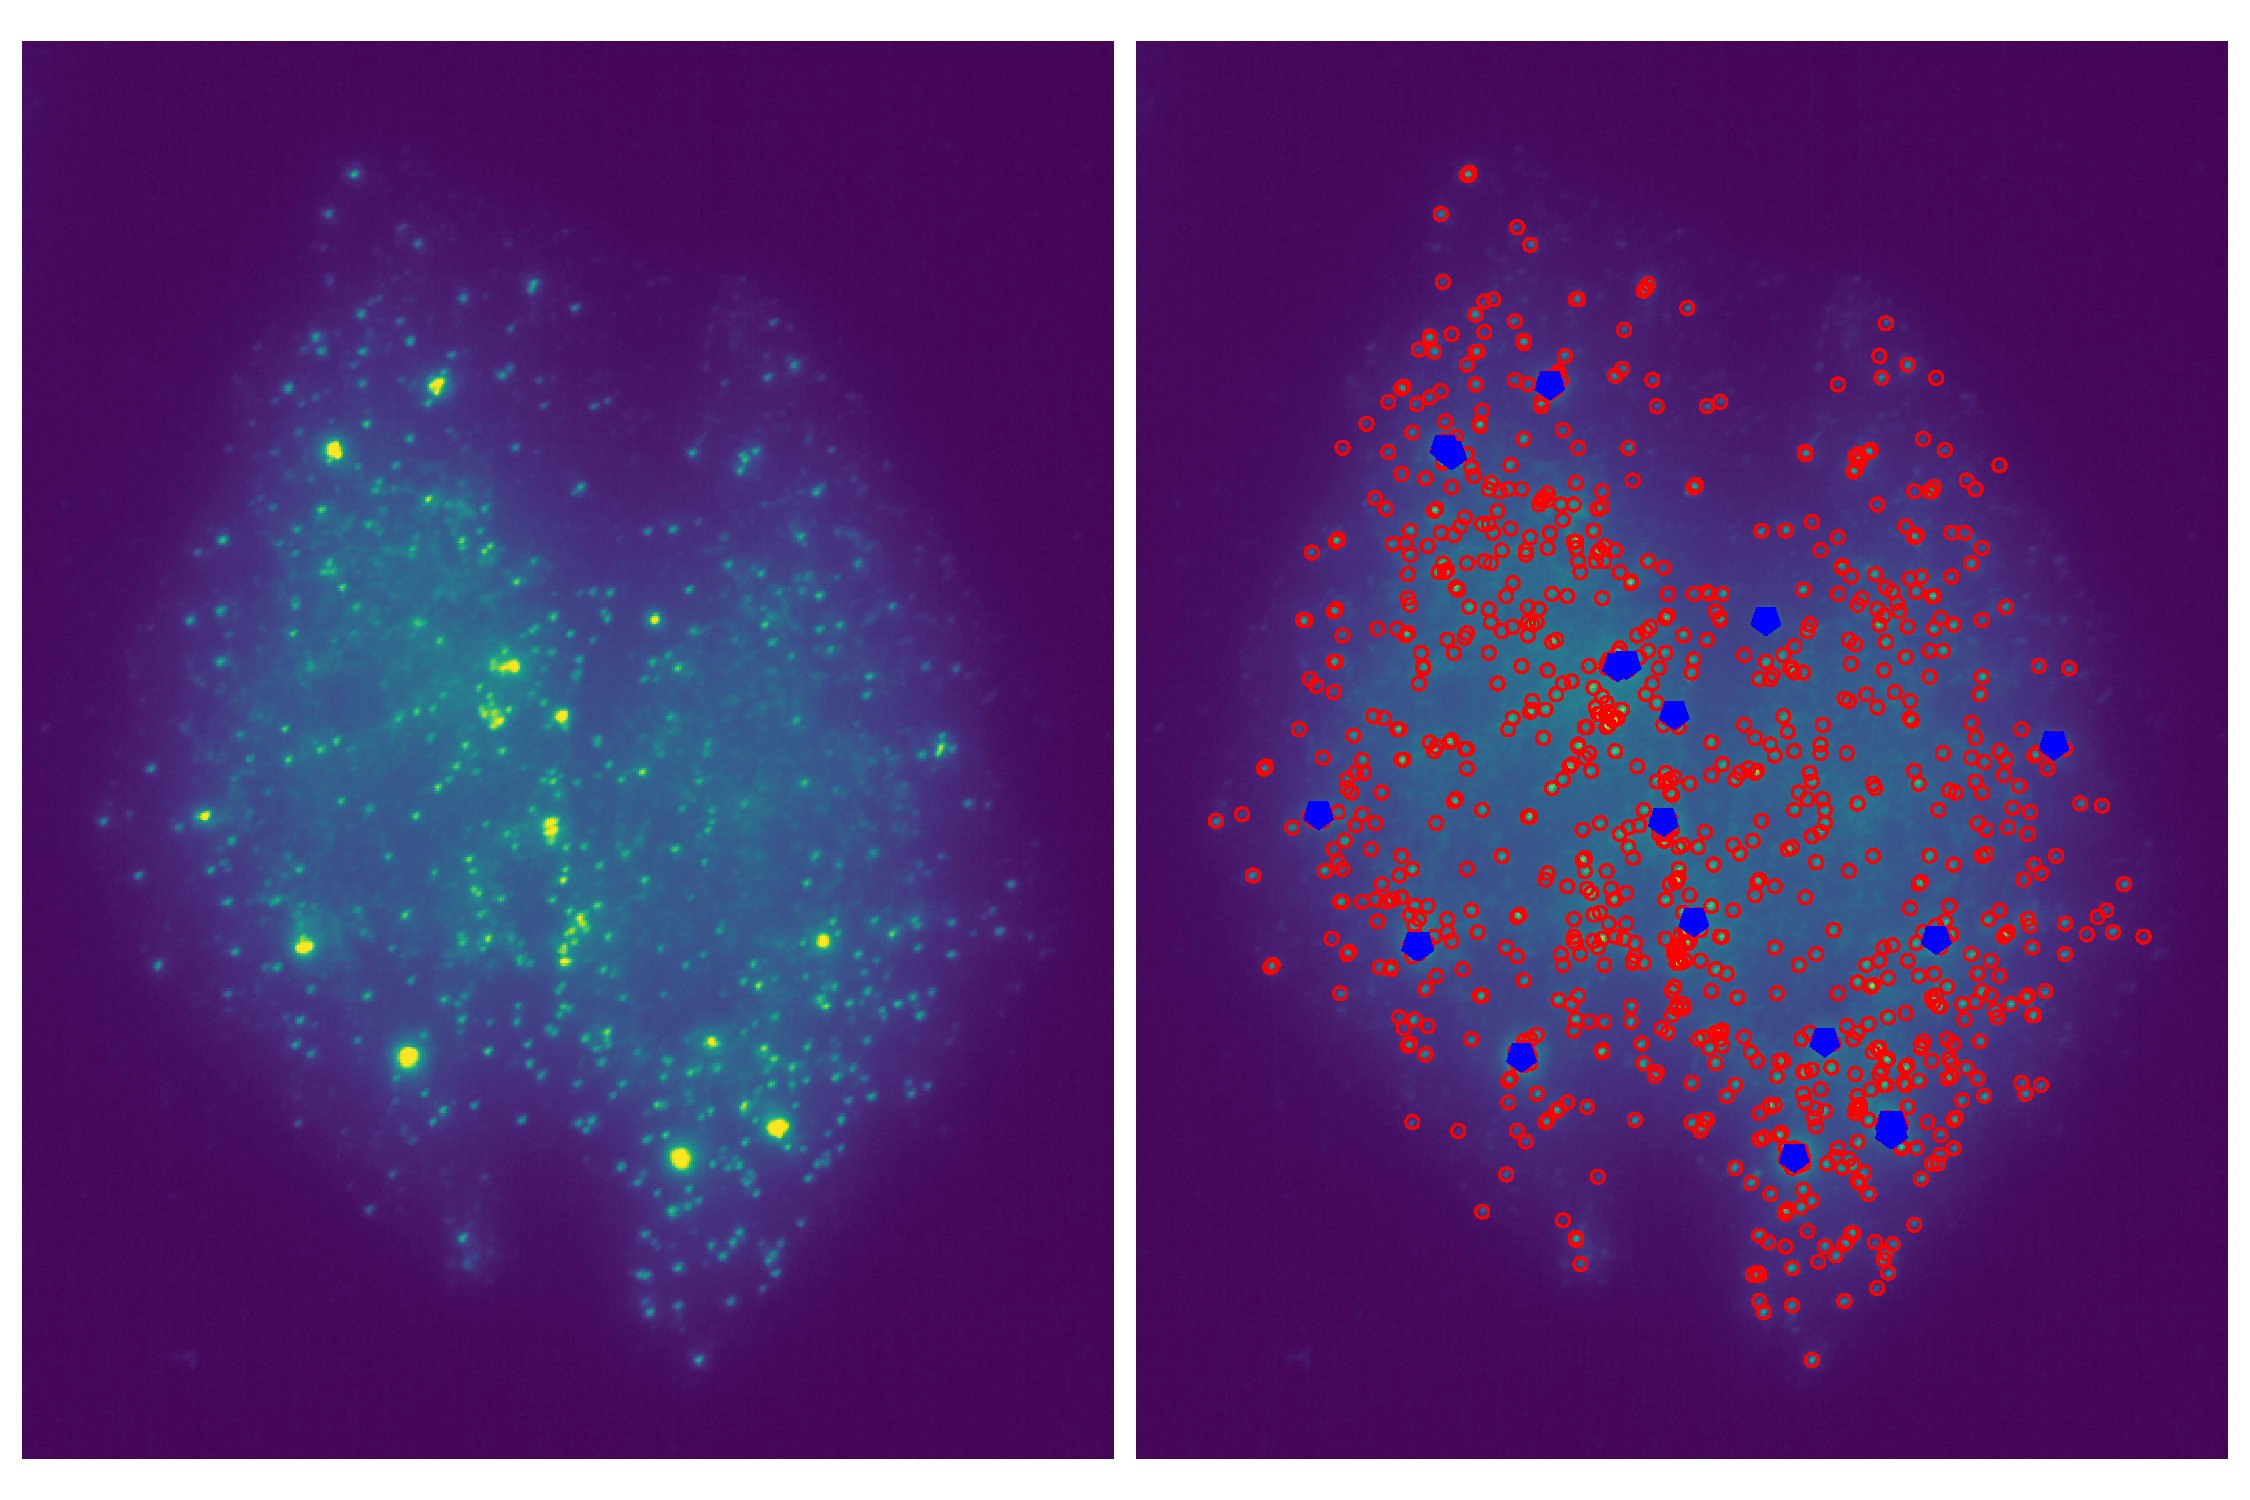
\includegraphics[width=1\textwidth]{figures/chapter2/cluster_detection_results}
	\caption{Detection results.
	(\textit{Left}) Original smFISH image.
	(\textit{Right}) Spots in \textit{red} and clusters in \textit{blue}, detected with \emph{bigfish.detection}}
    \label{fig:detection_results}
\end{figure}

\subsection{Problem description}
%\subsection{Extract spot coordinates from an image}
\label{subsec:detection}

%The aim of spot detection is to extract an array of spatial coordinates from an image with identifiable point sources.
From an image with identifiable point sources, the aim of spot detection is to extract an array of spatial coordinates corresponding to the spot centers. This task is performed in two or three dimensions, depending of the input image.

%Detecting an object as small as an \ac{RNA} molecule implies some constraints.
Detecting an object as small as an \ac{RNA} molecule faces several challenges.
\begin{enumerate}
\item The optical system does not capture the original light signal emitted by the fluorescence probes, but its convolution with a Point-Spread-Function (\ac{PSF}).
In this thesis, I will assume that the \ac{PSF} can be approximately described by a Gaussian in 2 or 3 dimensions. 
Such simplification is reasonable for a detection with pixel accuracy, given a good Signal-to-Noise-Ratio (\ac{SNR}).
\item As we can observe in Figure~\ref{fig:detection_results}, a \ac{smFISH} image often presents a background fluorescence, stemming from reporter molecules that are not specifically binding to target RNA and which are uniformly distributed in the cytoplasm. In 2D images, we thus observe that the background signal is roughly proportional to the local height of the cell. 
\item In addition, we can observe noise that actually resembles the signal we wish to detect, but at lower intensity. 
\item Both signal and noise can be highly heterogeneous and vary between images and between cells inside the same image
\item Depending on the density and the localization patterns, RNA molecules might be in close proximity: they might form clusters, for which no individual spots are distinguishable. In this case, the detection of individual RNA molecules might not be possible without simplifying assumptions. 
\end{enumerate}

% \noindent
% We can observe two types of noise:
% \begin{itemize}
% 	\setlength\itemsep{0.1em}
% 	\item At the \ac{FoV} level, the noise from the optical setup itself and the experimental conditions.
% 	\item At the cellular level, the difference in the autofluorescence of the observed samples.
% \end{itemize}

In the context of a high content screening, a large number of images are acquired, with various biological samples or conditions. For this reason, heterogeneity regarding pixel intensity and spot distributions represent a serious problem. At the same time, the number of images is such that we cannot reasonably manually adapt parameters for individual images (let alone individual cells). 
%For this reason, heterogeneity regarding pixel intensity and spot distributions represent a 
%This leads to potentially heterogeneous pixel intensity and spot distribution across different images.
%Spot detection can be really challenging.
It thus requires a robust approach to tackle this problem and extract accurate coordinates of the spot positions.

\subsection{Related work}
\label{subsec:detection_related_work}

\subsubsection{Traditional approaches based on filtering and thresholding}

Spot detection, especially for fluorescent images, has been addressed by the scientific community through different approaches. Classical approaches usually rely on filtering approaches that specifically enhance spot-like features, and binarization by thresholding or maxima detection. 

\paragraph{Methods}

Most spot detection methods can be decomposed into 3 steps: reduction of noise, signal enhancement and signal thresholding~\cite{smal_quantitative_2010}. 

%A general review~\cite{smal_quantitative_2010} defines most detection frameworks with three steps: noise reduction, signal enhancement and signal thresholding.

A popular method to reduce noise while enhancing spot-like structures is the convolution with a Gaussian filter. Filtering enhances the structures that resemble the filter itself, while attenuating high-frequency noise. Under the assumption of a Gaussian \ac{PSF}, a Gaussian filter is supposed to be particularly efficient. Alternative methods for noise reduction and signal enhancement include wavelet-based filtering, where the signal is decomposed with the Wavelet transform and non-significant Wavelet coefficients are discarded~\cite{Olivo-Marin2002}. 

% As for the noise reduction, they detailed in particular Gaussian smoothing technique, a method we exploit ourselves in the next section, and wavelet-based filtering.
% The later consists in applying a wavelet transform to obtain a sparse representation of the image, modifying the wavelet coefficients and transforming back the image.
% For this inverse transformation, we only keep the largest wavelet coefficients that correspond to structural elements in the image.

Signal enhancement refers to the specific enhancement of spot-like structures. As the spots we aim at detecting are small with respect to all other structures in the image, a popular strategy is to remove spots by some filter operation $\psi$ and to consider the residue $g - \psi(g)$ for further processing, where $g$ is the prefiltered image from the first step. $\psi$ might be a Gaussian filter (thus leading to the classical Difference of Gaussian (DoG) filter~\cite{Lindeberg2015}) or a morphological filter, such as the h-dome image~\cite{smal_quantitative_2010}, or diameter openings~\cite{Walter2007}. 
An alternative consists in evaluating the second order derivative by calculating the Laplacian of Gaussian (LoG). It can be shown that this approach is closely related to the DoG filter~\cite{Lindeberg2015}.
%Alternative strategies include the exploitation of radial symmetries~\cite{bahry_rs-fish_2021}, and the evaluation of the second order derivative by calculating the Laplacian of Gaussian (LoG). It can be shown that the latter approach is closely related to the DoG filter~\cite{Lindeberg2015}. 
% Signal enhancement is then the most critical step.
% Seven unsupervised methods are compared, including techniques like top-hat filter, \ac{LoG} filter or h-dome transformation.
% This transformation is a reconstruction by dilation $\mathcal{B}(x, y)$ of the original image $f(x, y)$, from an image $f(x, y) - h$, with $h$ a positive constant.
% As a result, we can decompose the original image such that $f(x, y) = \mathcal{H}(x, y) + \mathcal{B}(x, y)$, with $\mathcal{H}(x, y)$ the h-dome image with the remaining spots and local intensity peaks.
% It can be interpreted as a local background subtraction technique that cut-off ''intensities of height h from the top, around local intensity maxima''.
% Unlike previous mentioned filters, it does not involve any shape or size parameter, but a height parameter $h$.
% Based on their experiment, authors favor this technique when a good detection performance is needed.

%However, when image quality is great and the \ac{SNR} high enough, all the detection methods tested in~\cite{smal_quantitative_2010} perform well.

The third step is binarization. This is usually achieved by either thresholding the enhanced image or identification of local maxima, usually followed by application of additional criteria, such as intensity (which is also a form of thresholding).  

These three steps can be complemented by additional post-processing methods to disentangle close spots and refine the positions of the detected spots by \ac{PSF} fitting or exploitation of radial symmetry ~\cite{bahry_rs-fish_2021}.

Overall, it can be said that smFISH usually provides high \ac{SNR} images for cell culture, and differences between these detection methods are often marginal~\cite{smal_quantitative_2010}. 

%In order to disentangle spots in close proximity, these three steps can be complemented by deblending algorithms, 

%In any case, there is usually one or several parameters that need to be set in order to identify the RNAs.  
% Finally, the signal thresholding discriminates the relevant spots from the noise. 
%
%, depending of the detection method applied.
%Supervised techniques are also discussed and evaluated like the training of an ADABOOST model~\cite{FREUND1997119} with Haar-like features.
%These methods appear to be accurate, even with low \ac{SNR} images, but require annotated data and a training stage.

% Review from~\cite{ruusuvuori_evaluation_2010} completes the analysis with additional algorithms: kernel-based methods, Otsu thresholding~\cite{Otsu_1979} or source extraction~\cite{bertin_sextractor_1996}.
% The later is mainly applied in astronomy.
% It thresholds an image where the background has been estimated then subtracted, before deblending adjacent spots.

%These three steps provide a list of coordinates 


\paragraph{Implementations}

In general, software for RNA detection can rely on several spot detection algorithms that are already implemented and  available in popular Python packages like \emph{scikit-image}~\cite{walt_scikit-image_2014} or \emph{astropy}~\cite{astropy_2018}.
Astropy community developed an affiliated package \emph{photutils}~\cite{larry_bradley_2020_4044744} with helpful functions for photometry of astronomical sources like \ac{PSF} matching or source detection. Software tools for RNA detection in Python can thus rely on these libraries. 

There are also existing dedicated software solutions for the detection of RNAs, implemented in the three ecosystems used in bioimage informatics: Java, Python and MATLAB. For instance, Icy (implemented in Java), proposes a wavelet-based method for spot detection~\cite{de_chaumont_icy_2012}, the ImageJ/FIJI plugin Trackmate (also implemented in Java) implements a blob detection pipeline with \ac{LoG} filters ~\cite{ershov_trackmate_2022}, the recently published RS-FISH~\cite{bahry_rs-fish_2021} proposes \ac{Dog} filters with refined localizations as a FIJI plugin~\cite{schindelin_fiji_2012} (implemented in Java). 
%Additional software focused on fluorescent image analysis, but not always in Python.
%They propose their own spot detection pipeline like Icy~\cite{de_chaumont_icy_2012} (with a wavelet-based method) or Trackmate~\cite{ershov_trackmate_2022} (with a blob detection method).
The recent Python library \emph{starfish}~\cite{perkel_starfish_2019} wraps existing \emph{scikit-image} functions;  the first FISH-quant version~\cite{mueller_fish-quant_2013} (implemented in MATLAB) includes a blob detection pipeline with a \ac{LoG} filter. This last pipeline is the one we implemented and improved in our work for \emph{bigfish.detection}.


\tw{There is a copy paste issue here.}
% More recently RS-FISH~\cite{bahry_rs-fish_2021} was released specifically for 3D spot detection with \ac{FISH} images.
% Developed in Java and exploiting radial symmetry, it presents a great subpixel accuracy, a fast runtime computation and robustness against anisotropic spot signal.
% After a \ac{DoG} filtering, we threshold the image to generate potential spot localizations.
% We then extract image gradients around each spot and correct them for anisotropy.
% Besides possible outliers that are filtered out, gradients should point toward a common center: the spot localization.
Besides the processing capabilities and the specific implementations, most of the cited solutions also come with graphical user interfaces, namely Icy, Trackmate, FISH-quant and RS-FISH. One important aspect of these GUIs is to manually adapt algorithmic parameters, in particular the detection threshold. 

% In addition to their code, authors released a plugin for Fiji software~\cite{schindelin_fiji_2012}.
% Such \ac{GUI}, is not new: Icy, Trackmate and FISH-quant also have one.
% Like these alternatives, it allows the user to manually tune parameters and find the optimal setup for his application.

This last point is a major limitation for us.
The need for parameter tuning is a critical bottleneck for scaling detection.
When we apply an algorithm to thousands of images, with noise and intensity heterogeneity, most parameters need to be set once (or automatically) and not recalibrated between images.
In particular most of the presented methods require a threshold or a size parameter at some point.

% add a detailed description of top-hat filter
% add reference top-hat filter and h-dome transformation
% add exemples from smFISH, seqFISH+ and MERFISH applications

\subsubsection{Learning-based methods}

Spot detection has also been addressed by recent deep learning methods.
Deep learning (or more generally computer vision), allows one to perform spot detection without the a-priori definition of filters, models and criteria, and prevent parameter tuning on a cell-by-cell or image-by-image basis at the cost of a training stage, thus implying the establishment of ground-truth data.

A first study~\cite{bouilhol_deepspot_2022} proposes to preprocess images to make spot intensity homogeneous.
A convolutional network (named DeepSpot) is trained to enhance spot signal to the same intensity.
The network has two main components: a \ac{CASO} module followed by a customized ResNet~\cite{He_2016}.
\ac{CASO} mixes standard convolution blocks with strided and atrous (or dilated) convolutions~\cite{Hamaguchi_2018}.
Small objects like spots do not contain enough semantic information to be captured.
Standard convolution blocks (with max pooling) are great to learn semantic information, but at the expense of lower intensity spots and a potential spatial information loss.
One the one hand, replacing the pooling layer with strided convolution compensates the lower intensity.
On the other, the use of atrous convolution increases receptive field and thus improves context information with a minimal spatial information loss.

Another model, DeepBlink~\cite{eichenberger_deepblink_2021}, is based on a U-Net architecture~\cite{Ronneberger_2015} and directly detects spots.
The U-Net component extracts intermediate features.
Then it maps the original image into \emph{grid-cells} (small bounding-boxes) for which model predicts the probability of a spot localization and the potential 2D coordinates.
Size of the \emph{grid-cell} is critical.
With a small size, too many cells might be empty, resulting in an imbalanced dataset for the classification head of the model.
On the opposite, with a larger size, one cell could contain multiple spots (for only one prediction per \emph{grid-cell}).
This process is directly inspired by the detection model YOLO~\cite{Redmon_2016_CVPR}.

\section{Scaling \ac{mRNA} detection}
\label{sec:method}

We now describe at depth the algorithms currently implemented in \emph{bigfish.detection}.

\subsection{Spot detection}
\label{subsec:spot_detection}

The method we use is directly adapted from the original version of FISH-quant~\cite{mueller_fish-quant_2013} and the blob detection algorithms~\cite{walt_scikit-image_2014}.
Detection is performed in 2D or 3D. Images are filtered in order to increase \ac{SNR}, then each spot is defined as a local maximum above a specific threshold.

\subsubsection{Filtering}

We apply a \ac{LoG} filter (Gaussian filter followed by a Laplacian).
This is a two-step algorithm that enhances the spot signals. 

The Gaussian filter smooths the image and removes the high frequency noise. By choosing the Gaussian weights, it gives maximal output if the image structure under the filter is perfectly correlated to a Gaussian \ac{PSF}. 
Consequently, we apply this operator at a single scale because we assume a unique size for the spots, defined by the optical system. 
By default, the size of the Gaussian kernel is thus set to match the expected size of the spot which is assumed to be known for a given experiment. % and should not prevent the user to scale the detection.

The Laplacian filter approximates the second derivative of the image. Indeed, spots are supposed to correspond to local minima of the second derivative. 
If we consider a 2D image $f(x,y)$, the \ac{LoG} filter consists in computing the second derivative of the smoothed image $L(x, y, \sigma^2)$:

\begin{equation}
	{\displaystyle \nabla^{2}L(x, y, \sigma^2) = \frac{\partial^{2}L(x, y, \sigma^2)}{\partial x^2} + \frac{\partial^{2}L(x, y, \sigma^2)}{\partial y^2}}
\end{equation}

\noindent
with $L(x, y, \sigma^2)$ the convolve image:

\begin{equation}
	{\displaystyle L(x, y, \sigma^2) = g(x, y, \sigma^2) * f(x, y)}
\end{equation}

\noindent
and $g(x, y, \sigma^2)$ the Gaussian kernel with a scale $\sigma^2$:

\begin{equation}
	{\displaystyle g(x, y, \sigma^2) = \frac{1}{2\pi \sigma^2} e^{-{\frac{x^{2} + y^{2}}{2\sigma^2}}}}
\end{equation}

An alternative filter is the \ac{DoG} filter.
We estimate the background of the image with a large Gaussian kernel, then we subtract it from the original image or one smoothed with a narrower Gaussian kernel.
\ac{LoG} and \ac{DoG} filters are closely related. 
As illustrated in Figure~\ref{fig:filters_detection}, both methods aim to remove the background noise and enhance the spot signal.

% reference LoG and DoG

\begin{figure}[h]
    \centering
    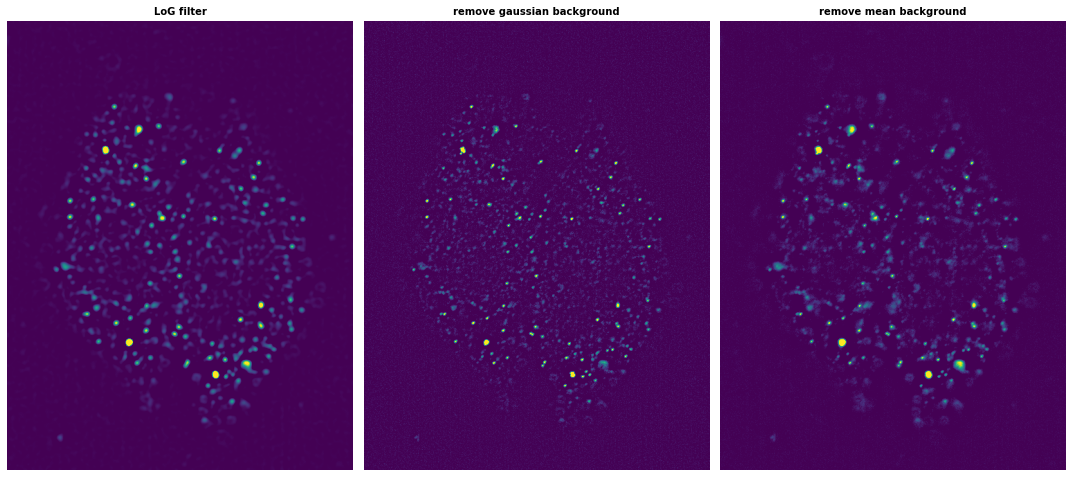
\includegraphics[width=1\textwidth]{figures/chapter2/filter_background}
    \caption{Filtered images with LoG filter (\textit{Left}) and DoG filter (\textit{Right})}
    \label{fig:filters_detection}
\end{figure}

\subsubsection{Peak detection}

A Local Maximum detection algorithm follows the filtering.
We apply a maximum filter on the \ac{LoG}-filtered image and compare the result to the original one.
A pixel with the same value in the original and filtered images is defined as a local maximum.
If, by chance, a spot has several identical pixels at its peak, we only keep one to define the spot coordinate.

% reference local maximum algorithm

\subsubsection{Thresholding}

At this stage, actual spots and noisy fluorescent blobs (e.g. off-site binding of oligos) are both detected.
From all previously detected local peaks, we only keep those above a specific threshold.
The problem is how to set this threshold. 
%A first limitation of spot detection algorithm appears with the choice of this threshold.
Manual setting of the threshold does not allow application of the detection method at a large scale, as the signal intensities can be very different between different images. Indeed, while image acquisition can be homogenized, the efficiency of the probes is necessarily heterogeneous. 
Thus, we use a heuristic technique to set a threshold per image in a automated way.

\begin{wrapfigure}{L}{0.35\textwidth}
	\begin{center}
		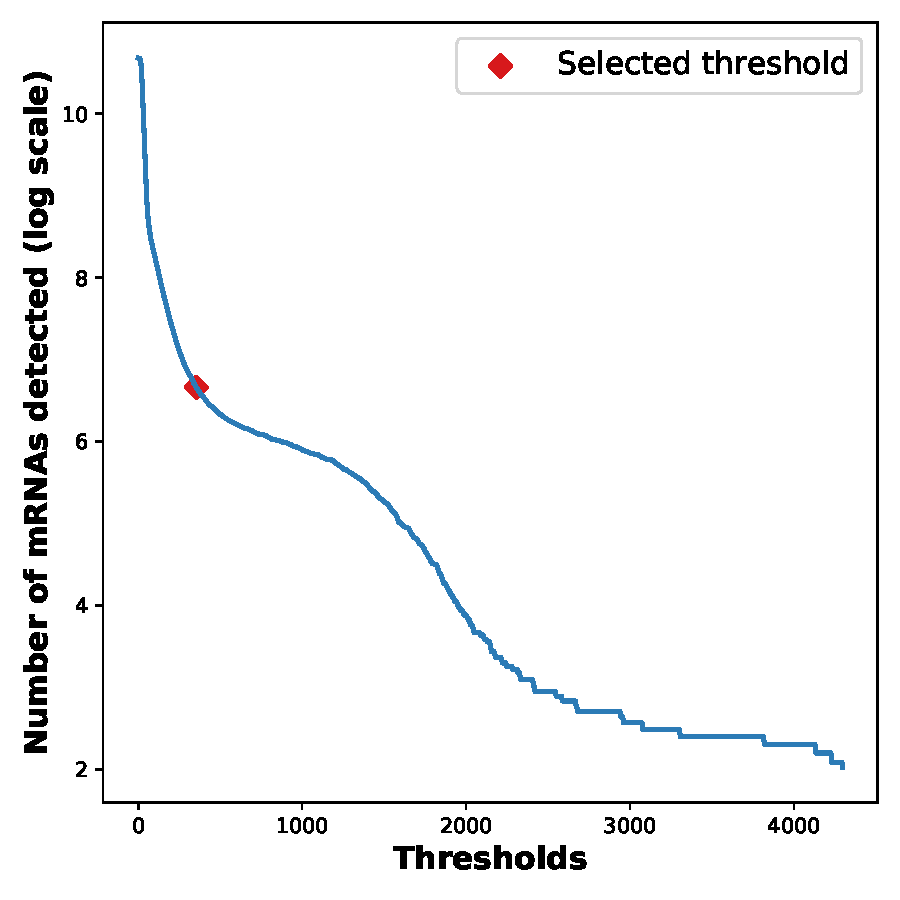
\includegraphics[width=0.33\textwidth]{figures/chapter2/elbow_curve_real}
	\caption{Elbow curve}
	\label{fig:elbow_detection}
	\end{center}
\end{wrapfigure}

We know that the major discriminative feature between spots originating from \ac{mRNA} and and those from off-site binding of oligos is their intensity: real mRNAs have significantly higher intensity values since an \ac{mRNA} molecule is targeted by multiple oligos. Conversely, the actual shape and size of true mRNAs and false positives is not necessarily different (see Figure \ref{fig:filters_detection}). 
%We assume that a \ac{mRNA} spot and a background fluorescent noise have different intensity distributions.
%The former have significantly higher intensity values since a \ac{mRNA} molecule is targeted by multiple oligos.
In the Figure~\ref{fig:elbow_detection}, we plot the relation between different thresholds and the number of selected spots (with a log scale).
We observe a sharp and monotone decrease in the number of detected spots with increasing detection threshold.
The \emph{spots} removed are mostly background noise at these low threshold levels.
Actual spots are too bright to be filtered out.
At the opposite, if we increase the threshold too much, we start removing real spots and the sensitivity of the detection decreases.

In addition, we assume that wrong detections due to noise are much more frequent than actual mRNAs. This is a reasonable assumption, as off-site binding of a low number of probes is frequent. This means that the decrease in spot number when the threshold increases should be large and relatively steady. As soon as the number of removed spots by a further increase drops dramatically (see red point in Figure ~\ref{fig:elbow_detection}), we can assume that we are reaching a point, where we have removed most of the low-intensity noise and start removing spots originating from real mRNAs. 
We can thus argue, that the sweet spot for the threshold is reached when the reduction in spot number is beyond this first steep decrease, and reaches the average value. This value is reached when the tangent's slope equals the average slope of the curve (for the first time). 
%For a good image quality, the adequate intensity threshold corresponds to a plateau in the elbow curve~\ref{fig:elbow_detection}.
We have observed that even if this plateau is less pronounced than in Figure ~\ref{fig:elbow_detection}, for instance if there is a particularly high level of noise, an abrupt change in the slope of the curve is still identifiable.
This difference of slope describes a clear separation between the regimes of overdetection and underdetection.

%In order to automatically set an optimal threshold, we geometrically find the plateau of the elbow curve in~\ref{fig:elbow_detection}.
%We select the threshold where the tangent's slope equals the average slope of the curve.
Additional elbow curves can be observed in appendix~\ref{sec:appendix_detection}, with different conditioning.\\

\begin{minipage}{0.9\textwidth}
\begin{lstlisting}[language=Python]
import bigfish.detection as detection

# spot detection with automated thresholding
spots, threshold = detection.detect_spots(
    images=smfish,
    return_threshold=True,
    voxel_size=(300, 103, 103),  # in nanometer
    spot_radius=(350, 150, 150))  # in nanometer
\end{lstlisting}
\end{minipage}

\subsection{Managing high spot density}
\label{subsec:dense_decomposition}

\tw{It was not so clear, why we need these 2 steps. I have tried to motivate this a bit ... please check whether you agree. }

A second challenge in spot detection is the presence of clustered spots and high density areas, like active transcription sites or \ac{RNA} foci.
The method described above in~\ref{subsec:spot_detection} works well with isolated spots.
When spots are agglomerated, they might not be possible resolve anymore.
%This is not clear: In addition, detection methods based on quick and sharp changes in terms of pixel intensity might fail to detect a spot in a bright and uniform region. (I propose to drop the sentence)
In practice, an accumulation of spots looks like a large and bright fluorescent region where our detection will underestimate the number of individual spots.

One option might be to use blob detection at different scales~\cite{walt_scikit-image_2014}, which would allow to identify these clusters as one spot. However, we could still not represent them as an agglomeration of individual spots. 
%Using a different (and larger) scale, a blob detection algorithm~\cite{walt_scikit-image_2014} might help to detect the cluster as a bigger spot.
%However such method does not allow to decompose the cluster in individual spots.
In \emph{bigfish.detection} we adapt the solution proposed in a previous version of MATLAB FISH-quant~\cite{mueller_fish-quant_2013, samacoits_computational_2018}.
We handle high spot density regions in two independent steps:

\begin{itemize}
	\setlength\itemsep{0.1em}
	\item In order to deal with \ac{RNA} underdetection in dense regions, we identify potential dense regions and decompose them into individual spots. This step increases the number of detected spots in the image (see figure~\ref{fig:dense_decomposition}).
	\item For subsequent analysis of the presence / number of clusters, we detect \ac{RNA} clusters by applying a clustering algorithm to the \ac{RNA} point cloud. This step can be performed with or without the dense region decomposition. 
\end{itemize}

While somehow related, we stress that the first step tackles a technical issue of underdetection, while the second step allows us to separately define \ac{RNA} clusters for further analysis, as the presence / number of clusters is an important feature of \ac{RNA} localization. 

\subsubsection{Dense region detection}

\begin{wrapfigure}{R}{0.35\textwidth}
	\begin{center}
		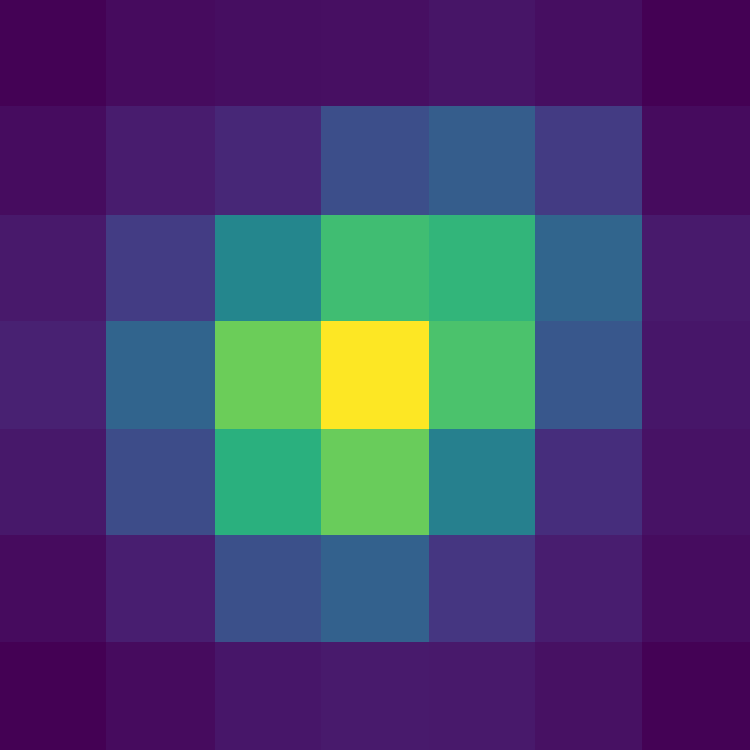
\includegraphics[width=0.33\textwidth]{figures/chapter2/reference_spot}
	\caption{Reference spot}
	\label{fig:reference_spot}
	\end{center}
\end{wrapfigure}

The first step consists in localizing regions in the image with a probable cluster of spots.
We know that for such regions our detection might miss several spots.

We remove the low-frequency noise from the image by subtracting its background intensity.
The latter is approximated with a large Gaussian filtering.
From this image we then extract the detected spots and compute the median spot signal.
This median signal %is used as an \ac{RNA} prototype and 
allows us to define criteria for the identification of high density regions. 
%threshold to filter the candidate regions with potential clustered spots.
We expect high density regions to be brighter than individual spots, so they should at least be brighter than the median spot intensity. A second criterion is the size of the regions.
Furthermore, they should be larger than an individual spot.
To match these criteria, we first threshold the denoised image with the median spot intensity, then we apply a connected component algorithm~\cite{wu_connected_component_2005} to the binary mask obtained.
Each group of connected pixels represents a region.
Because the mask is the result of a thresholding above the median spot signal, every region (or connected component) with at least 2 pixels are larger and brighter than the median spot for this image.

\subsubsection{Dense region decomposition}

%So far, the candidate regions can be actual clusters or simply one individual spot, brighter than the average.
\tw{check whether the first sentence is correct}
The candidate regions can contain clearly distinguishable spots, but they can also contain a one large spot, corresponding to an agglomeration of very close \ac{RNA}s. 
We reuse the denoised image and aggregate the detected spots to compute a reference spot like in Figure~\ref{fig:reference_spot}.
By default this reference is the median spot, but another percentile can be chosen.
We fit a Gaussian signal on the reference spot.
This model can then be used to simulate new spots.

The decomposition process consists in populating our candidate regions by simulating as many spots as possible until we match the pixel intensity we observe.
Starting with an empty image, we iteratively add a new simulated spot in the region until we minimize the residual sum of square (RSS):

\begin{equation}
	{\displaystyle \operatorname{RSS} = \sum _{x, y}(\hat{f}(x, y) - f(x, y))^{2}}
\end{equation}

\noindent
with $\hat{f}(x, y)$ the simulated image intensity and $f(x, y)$ the denoised image.

\begin{figure}[h]
    \centering
    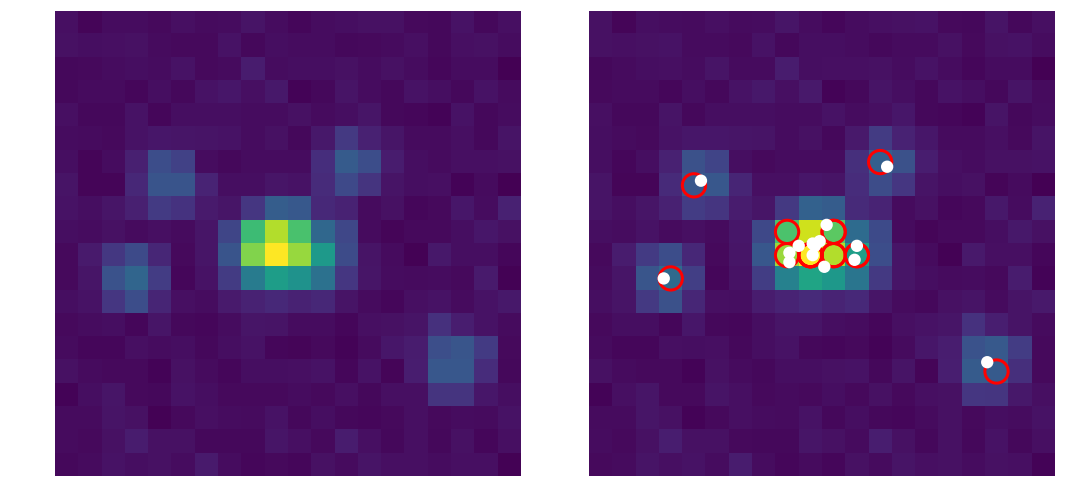
\includegraphics[width=1\textwidth]{figures/chapter2/plot_dense_decomposition}
    \caption{Decomposition results.
	(\textit{Left}) Original smFISH image zoomed in a dense region.
	(\textit{Right}) Detected spots in \textit{red} and actual clustered spots in \textit{white}}
    \label{fig:dense_decomposition}
\end{figure}

\subsubsection{Cluster detection}

\tw{Again, check that the first sentence is correct.}
The second (independent) step consists in applying a clustering algorithm on the spatial positions, in order to identify clusters according to a clearly understandable, biological meaningful definition, only based on spatial coordinates. 
%Once we detect a \ac{RNA} point cloud, with or without the decomposition step, we look for \ac{RNA} clusters.

To this end we use a DBSCAN algorithm~\cite{ester_density-based_1996, scikit-learn}.
Two parameters need to be set: a minimum number of spots $k$ and a threshold distance $d$.
Every pair of \ac{RNA}s closer than $d$ are connected.
If an \ac{RNA} is connected to at least $k$ neighbors \ac{RNA}, it's a \emph{core sample} and with its connections it defines a cluster.
Such a method allows us to detect clusters as ''areas of high density separated by areas of low density''\footnote{\url{https://scikit-learn.org/stable/modules/clustering.html}}.

Different users might may have a different definition of what they expect to be a cluster.
For the rest of the manuscript and throughout our studies, we usually consider a minimum group of 4 or 5 \ac{RNA}s within a radius of 350nm.
These are the default parameters in \emph{bigfish.detection} and the ones we use in Figure~\ref{fig:detection_results}.\\

\begin{minipage}{0.9\textwidth}
\begin{lstlisting}[language=Python]
import bigfish.detection as detection

# dense decomposition
spots_post_decomposition, _, _ = detection.decompose_dense(
    image=smfish,
    spots=spots,
    voxel_size=(300, 103, 103),  # in nanometer
    spot_radius=(350, 150, 150))  # in nanometer

# cluster detection
spots_post_clustering, clusters = detection.detect_clusters(
    spots=spots_post_decomposition,
    voxel_size=(300, 103, 103),  # in nanometer
    radius=350,  # in nanometer
    nb_min_spots=4)
\end{lstlisting}
\end{minipage}

\subsection{Going beyond pixel accuracy}
\label{subsec:subpixel}

Two additional methods for reaching subpixel accuracy have been integrated in FISH-quant. They were already present in the first version of FISH-quant ~\cite{mueller_fish-quant_2013}.
%Two additional methods already present in the first version of FISH-quant~\cite{mueller_fish-quant_2013} have been implemented in \emph{bigfish} as it is.

\subsubsection{Subpixel fitting}

So far, the spot detection and the dense region decomposition and the cluster detection return coordinates with pixel accuracy.
In our applications, we were only interested in overall \ac{RNA} distribution, but for some applications, subpixel accuracy is critical.
%This can lead to a small inaccuracy, irrelevant for our own studies, but potentially critical for some users.
Such error can be observed in the Figure~\ref{fig:dense_decomposition} between the detected spots (with pixel accuracy) and the ground truth (with subpixel accuracy).

The possibility to refine the coordinate on individual spots solves this limitation.
For this, we loop over the detected spots, crop the image and fit a gaussian signal on each of them individually.
We then correct the spot coordinates with the coordinates of the fitted gaussian.

\tw{What do you mean with "negative results"? }
Obviously, such method might return negative results in high density areas when spots can't be resolved.\\

\begin{minipage}{0.9\textwidth}
\begin{lstlisting}[language=Python]
import bigfish.detection as detection

# subpixel fitting
spots_subpixel = detection.fit_subpixel(
    image=smfish,
    spots=spots,
    voxel_size=(300, 103, 103),  # in nanometer
    spot_radius=(350, 150, 150))  # in nanometer
\end{lstlisting}
\end{minipage}

\subsubsection{Spot colocalization}

\begin{wrapfigure}{R}{0.35\textwidth}
	\begin{center}
		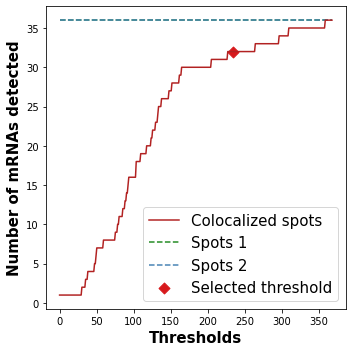
\includegraphics[width=0.33\textwidth]{figures/chapter2/colocalization_elbow}
	\caption{Threshold impact on colocalization}
	\label{fig:elbow_colocalization}
	\end{center}
\end{wrapfigure}

Another method requested by the community is the possibility to detect adjacent spots in different channels then match their coordinates.
%Our implementation is based on the one developed in the recent work from~\cite{CORNES_2022}.
This could be the same \ac{RNA} detected with two different fluorescent probes or techniques in order to validate experimental protocols, or different \ac{RNA} for which we would like to investigate the co-localization. 
As an example, in the Figure~\ref{fig:elbow_colocalization}, we detect colocalized spots between a sample of spots detected with pixel accuracy and the same sample with subpixel accuracy.

Our implementation is based on the methods published by ~\cite{CORNES_2022}.
First we compute the euclidean distance matrix between the two sets of spot coordinates, then we solve a linear sum assignment problem~\cite{crouse_linear_assignment_2016, 2020SciPy-NMeth}.
We obtain a matching between the two sets of spots, that minimizes the overall euclidean distance between assigned pairs.
Finally, we only keep pairs with a distance below a specific threshold.
The Figure~\ref{fig:elbow_colocalization} illustrates the impact of the threshold parameter on the number of colocalized spots.
Like for the spot detection, we implement our heuristic~\ref{subsec:spot_detection} to infer an optimal threshold if none is provided.\\

\begin{minipage}{0.9\textwidth}
\begin{lstlisting}[language=Python]
import bigfish.multistack as multistack

# spot colocalization
(spots_1_colocalized, spots_2_colocalized,
 distances) = multistack.detect_spots_colocalization(
	spots_1=spots_crop,
	spots_2=spots_subpixel_crop,
	voxel_size=(300, 103, 103))  # in nanometer
\end{lstlisting}
\end{minipage}

% \cite{lagache_statistical_2015}
% Colocalization methods are traditionally divided into pixel-based methods
% that measure global correlation coefficients from the overlap between pixel
% intensities in different color channels, and object-based methods that first
% segment molecule spots and then analyze their spatial distributions with
% second-order statistics.

\section{Evaluation with simulated spots}
\label{sec:detection_evaluation}

Finally we describe our evaluation of \emph{bigfish.detection}.
In addition to qualitative assessment of spot detection throughout our studies, we quantify the error from simulated images.
Performances for both spot and cluster detections are measured with different image qualities.

\subsection{Simulations}
\label{subsec:simulation}

To measure the error of a spot detection we need a ground truth.
A manual annotation of a regular 3D \ac{smFISH} image is intractable : such a strategy would be extremely time-consuming and prone to human error.
The alternative is to simulate realistic images of spots under different noise conditions in order to assess the performance of our algorithms and to study its limitations depending on image quality.
To this end, we built the simulation package \emph{simfish} that allows us to precisely control the level of noise and the number of spots we want to simulate in the image.

\subsubsection{Spot simulation}

The simulation process aims to return both an image and the ground truth coordinates of the spots we simulated.

\noindent
Our images are generated with three main steps:

\begin{enumerate}
	\item We randomly draw the number of spots and their localization.
	This is our ground truth.
	The number of spots is sampled from a Poisson distribution and the localizations from a uniform distribution all over the frame.
	Alternatively the number of spots can be set manually.
	\item For each spot in the image we simulate its pixel intensity.
	Instead of directly sample the intensity value from a Gaussian distribution, we reuse the simulation process from~\cite{bahry_rs-fish_2021}.
	With a Gaussian distribution centered on every spot, we simulate the average number of photons collected by each pixel in the image.
	The amplitude and the standard deviation of this Gaussian signals are manually or randomly predetermined.
	The final intensity of every pixel is then sampled from a Poisson distribution with the number of photons as expectation.
	\item (Optional) We add a background white noise to the entire image.
	It follows a Normal distribution centered around a predefined noise level.
\end{enumerate}

% add a schema of the cluster simulation process if necessary

The process detailed above generate spots with pixel accuracy.
A simulation with a subpixel accuracy follows the same steps, but with a larger image (4 to 20 times larger).
Before saving the image and the ground truth, it is downsized by local averaging.
The ground truth coordinates are adapted accordingly.

In order to produce a noisier image we can decrease the ratio between the spot amplitudes and the background noise.
A second option is to increase the variance of the different parameters: spot standard deviation and amplitude, background noise standard deviations.

\subsubsection{\ac{SNR}}

We can tune the different parameters mentioned to simulate spots with an increasing level of difficulty to detect.
To quantify the noise of an image and graduate the challenge it offers in terms of detection, we compute its \ac{SNR} for every spot.

\noindent
For a 2D image, we define the $\operatorname{SNR}$ of an image as the median of the $\operatorname{SNR_i}$ we compute for each spot $i$, such that:

\begin{equation}
	{\displaystyle \operatorname{SNR_i} = \frac{\max(a(x, y)) - \mu(b(x, y))}{\sigma(b(x, y))}}
\end{equation}

\noindent
with $\mu(.)$ the mean, $\sigma(.)$ the standard deviation, $a(x, y)$ the cropped spot image and $b(x, y)$ the spot background (a crop twice larger than the spot image).

In consequence, our measure of noise is based on the spot coordinates.
We quantify how distinct the spot is from its background.
A spot with a low amplitude or a noisy background will decrease the \ac{SNR} of the image.
To correctly quantify the image noise during our evaluation, we use the ground truth coordinates of the spots to compute the \ac{SNR}.
Indeed, a noisy image would impact the detection and bias the measure of noise itself.
We simulate different images with a range of \ac{SNR} between 2 and 26.
The higher the \ac{SNR} is, the better.

For example, in Figure~\ref{fig:spot_detection_high_noise} we simulate an extreme case with a highly noisy image (\ac{SNR} below 5).
On the right panel we can observe some contrasted background blobs misdetected as spot.
Despite a small amount of false positives, the detection remains correct in this badly conditioned image.

\begin{figure}[h]
    \centering
    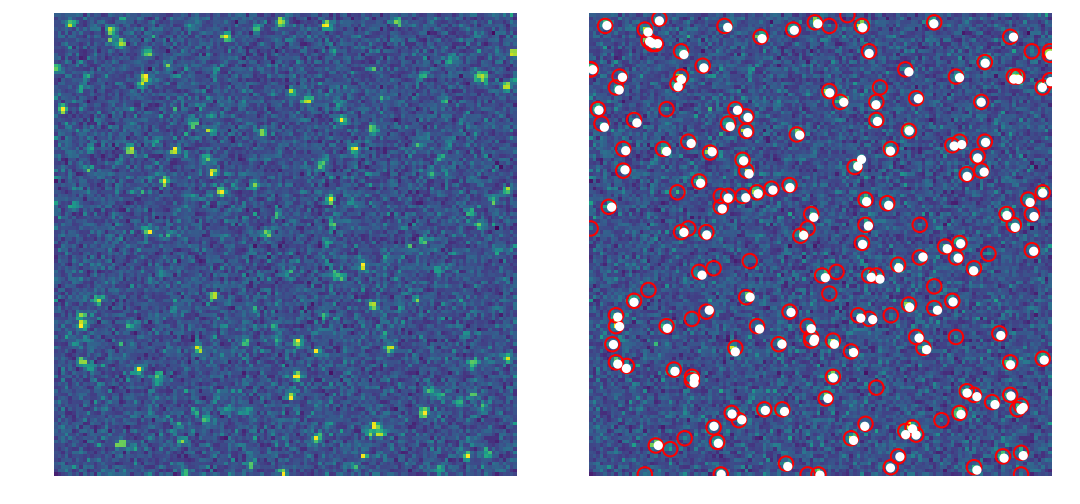
\includegraphics[width=1\textwidth]{figures/chapter2/plot_spot_detection}
    \caption{Noisy spot simulation with \emph{simfish}.
	(\textit{Left}) Original simulated image.
	(\textit{Right}) Detected spots in \textit{red} and actual spots in \textit{white}}
    \label{fig:spot_detection_high_noise}
\end{figure}

\subsubsection{Cluster simulation}

The user can also decide to simulate clusters.
In this case, the first step of our simulation process is adapted.
First the number of clusters and the number of spots per cluster are drawn from a Poisson distribution (or manually set).
The cluster centers are then localized like spots, with a uniform distribution over the entire image, or fixed at the center of the frame.
Finally, different spot localizations are randomly generated around the centers, using polar coordinates.
The result can be observed in Figure~\ref{fig:dense_decomposition} which is actually a simulated cluster.
In addition, several simulations are available in appendix~\ref{sec:appendix_simulations_spots}, with different conditioning.\\

\begin{minipage}{0.9\textwidth}
\begin{lstlisting}[language=Python]
import simfish as sim

# image simulation
image, ground_truth = sim.simulate_image(
	ndim=3,
	n_spots=100,
	image_shape=(128, 128),
	voxel_size=(100, 100, 100),  # in nanometer
	sigma=(150, 150, 150),  # in nanometer
	amplitude=5000,
	noise_level=300)
\end{lstlisting}
\end{minipage}

\subsection{Results}
\label{subsec:detection_results}

We simulated batches of 100 images with high, medium and low noise levels (roughly, with a \ac{SNR} below 5, between 5 and 15 and above 15).

\subsubsection{Impact of noise}

Our method is overall pretty robust.
If the image quality deteriorates, with a lower \ac{SNR} for example, our algorithms can return a moderate overestimation of detected spots.
This overestimation is estimated below 5\% and 10\% for images with a low or medium \ac{SNR} value, respectively.

These measures are illustrated on the left panel of Figure~\ref{fig:detection_error}.
We compared the number of spots detected with the actual number of spots simulated.
Each dot corresponds to one image.
For each noise regime, 100 images are generated.
Above the plain line, the detection overestimates the number of spots.
Logically, these overestimations increase with the noise level (and decrease with increasing \ac{SNR}).

On the right panel, we summarize the impact of noise with our detection technique.
Each dot represents again an image, with 100 simulated spots and a varying level of noise.
Below a \ac{SNR} of 5, with poorly contrasted spots, a fully automated detection might remain challenging.

\begin{figure}[h]
    \centering
    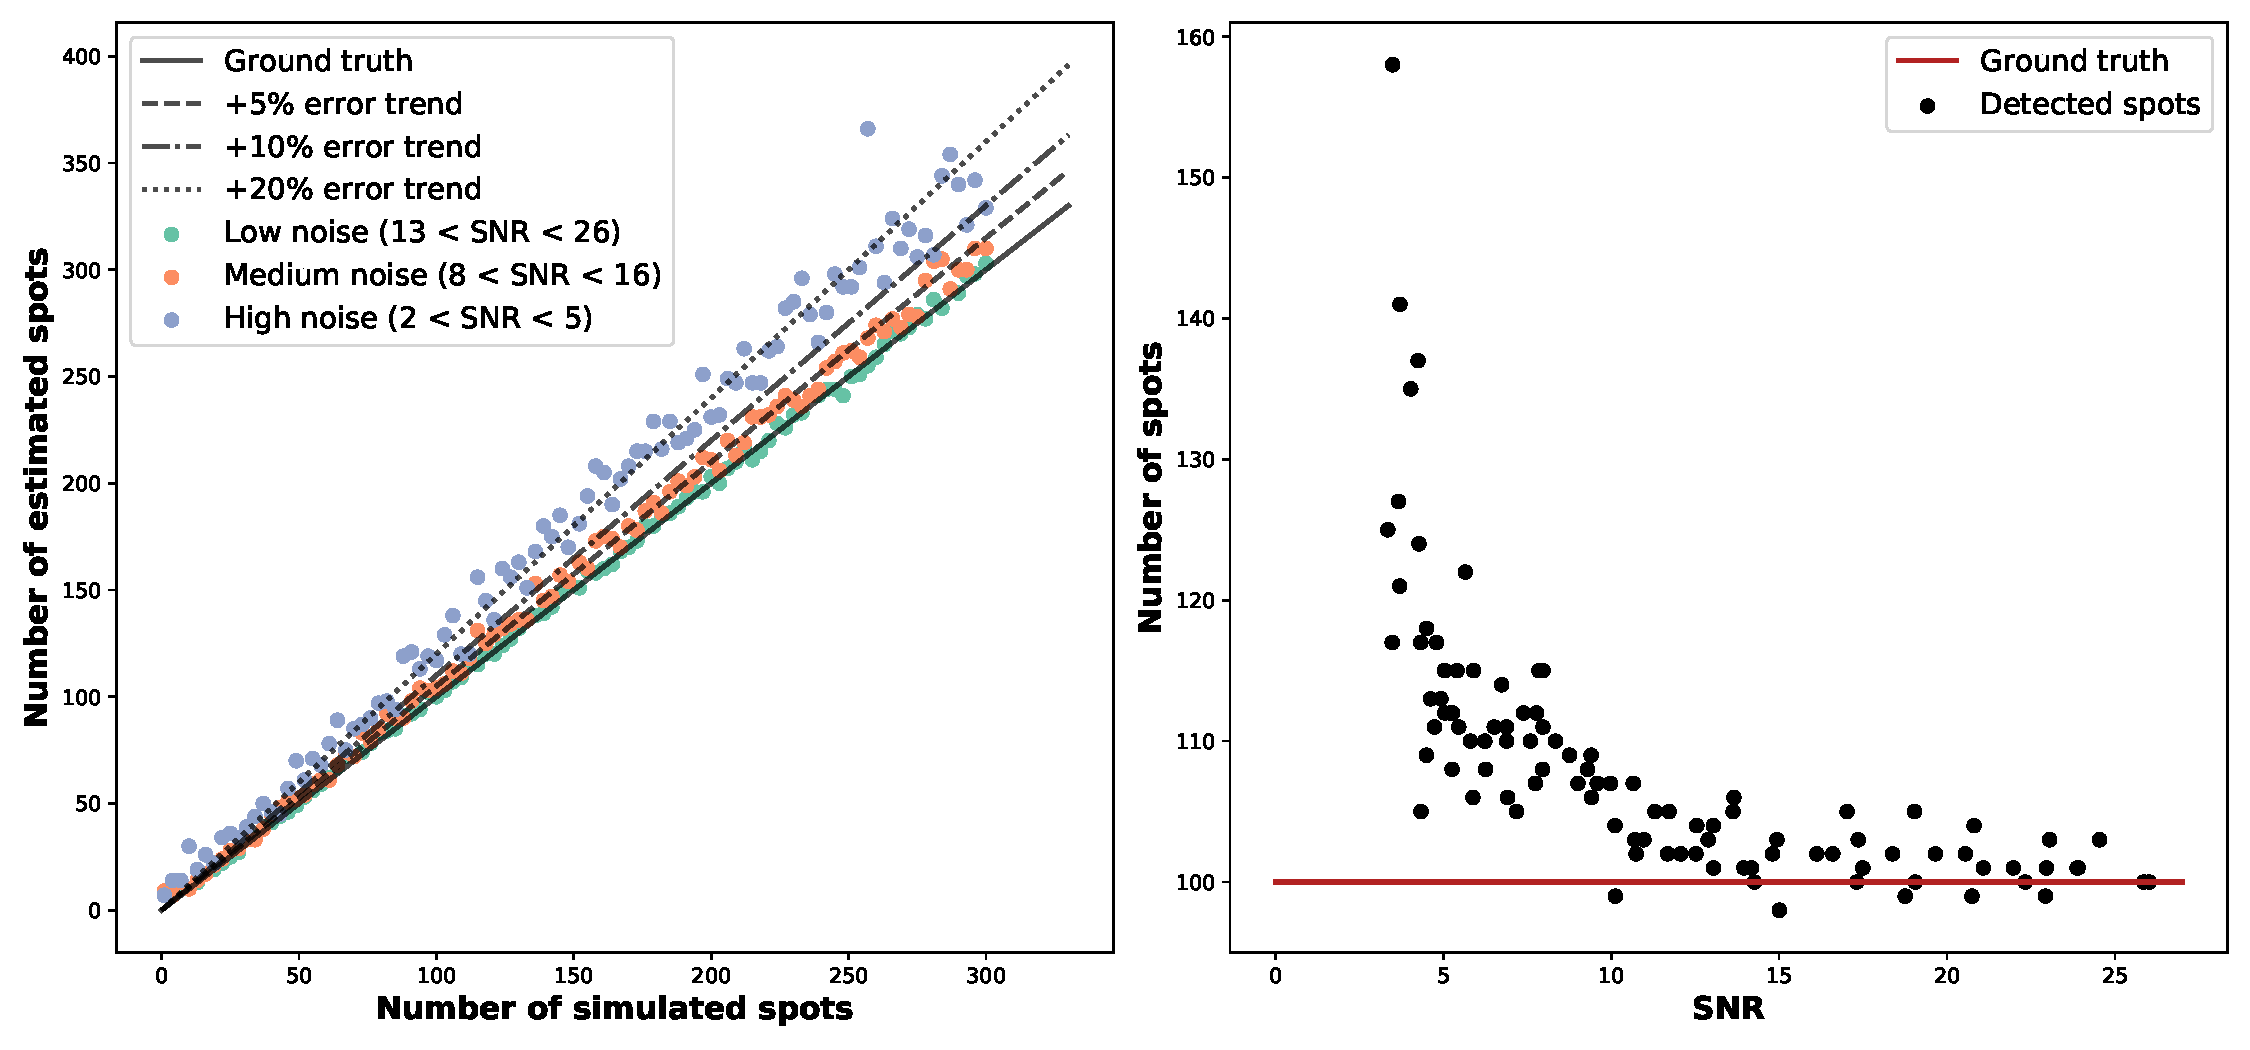
\includegraphics[width=1\textwidth]{figures/chapter2/fused_spot_detection_noise}
    \caption{Impact of noise on automated detection.
	(\textit{Left}) Number of detected spots for different numbers of simulated spots.
	(\textit{Right}) Number of detected spots for different levels of noise (with 100 simulated spots)}
    \label{fig:detection_error}
\end{figure}

\subsubsection{Accuracy of the cluster detection}

We simulate images with a unique cluster in order to test the performance of our method to decompose the dense regions and detect the clusters.
Such images can be observed in appendix~\ref{sec:appendix_simulations_spots}.
In Figure~\ref{fig:cluster_results} we report the number of spots we estimate in the clusters.
Each dot represents an image with a cluster.
Our decomposition is quite robust with the noise level, even with the lower \ac{SNR} values.
However, for the largest clusters, with 15 spots or more, we tend to slightly underestimate the number of spots.
In this case, the average error is 1.6.
In comparison, with 5 spots and 10 spots per cluster, we measure an average error of 0.83 and 0.82, respectively.

\begin{figure}[h]
    \centering
    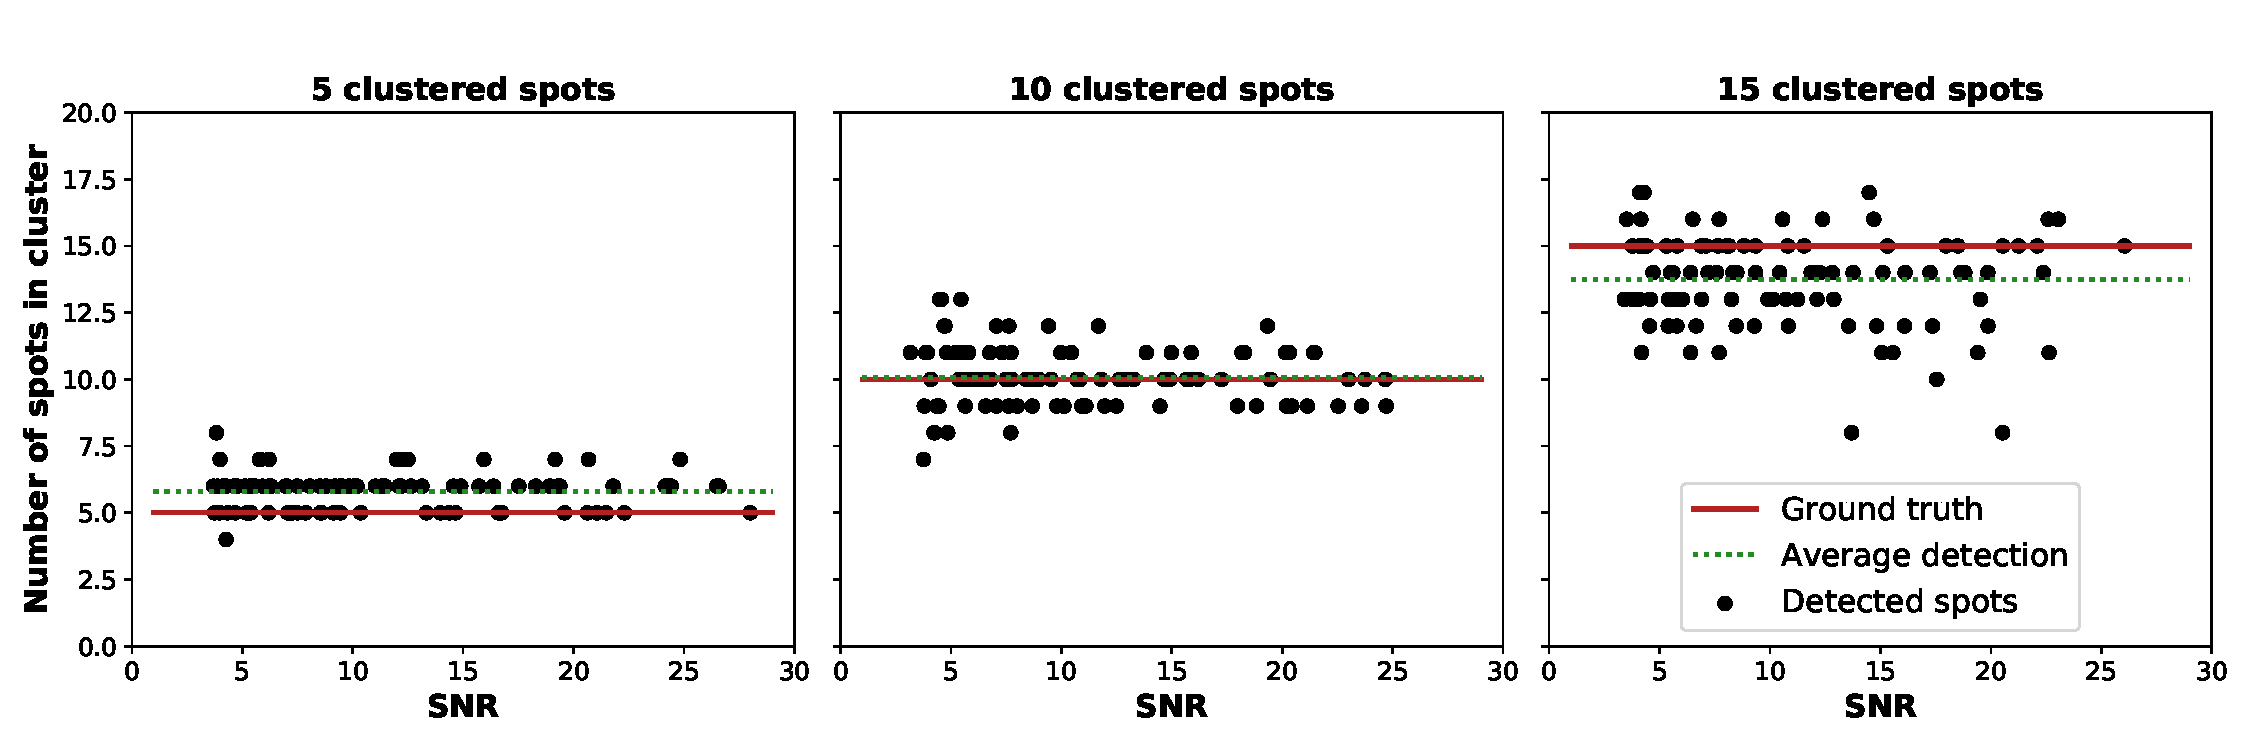
\includegraphics[width=1\textwidth]{figures/chapter2/cluster_along_noise}
    \caption{Dense region decomposition evaluation.
	 Number of spots estimated per cluster for different levels of noise and respectively 5 (\textit{left}), 10 (\textit{center}) or 15 (\textit{right}) simulated spots per cluster}
    \label{fig:cluster_results}
\end{figure}

%\subsubsection{Performance assessment - an open problem in smFISH analysis}

%We

\subsection{What if the \ac{PSF} is not Gaussian?}
\label{subsec:psf}

In this chapter we assume our \ac{mRNA} spots can be modelled with a Gaussian signal.
This simplification was relevant during my PhD and did not lead to exaggerated errors in our different analysis.
However, it is always possible to exploit a more complex \ac{PSF} to fit with a specific spot signal.
To this end, the former \emph{psf} package\footnote{\url{https://github.com/cgohlke/psf/}} allows to generate more complex \ac{PSF} for specific fluorescent microscopic experiments.
Letting the user choose between different \ac{PSF} is an improvement that could be implemented in a future version of \emph{bigfish.detection} and \emph{simfish}.
In particular, this would modify the way we generate spot signal in our image simulations or in the decomposition of dense regions.

Eventually, if the \ac{PSF} differs greatly from a Gaussian signal, the spot detection itself could be impacted.
Indeed, two \ac{PSF}s from close spots could interfere and make the local peaks less distinct.

% potential references in PSF
% Electromagnetic diffraction in optical systems. II. Structure of the image field in an aplanatic system. B Richards and E Wolf. Proc R Soc Lond A, 253 (1274), 358-379, 1959.
% Focal volume optics and experimental artifacts in confocal fluorescence correlation spectroscopy. S T Hess, W W Webb. Biophys J (83) 2300-17, 2002.
% Electromagnetic description of image formation in confocal fluorescence microscopy. T D Viser, S H Wiersma. J Opt Soc Am A (11) 599-608, 1994.
% Photon counting histogram: one-photon excitation. B Huang, T D Perroud, R N Zare. Chem Phys Chem (5), 1523-31, 2004. Supporting information: Calculation of the observation volume profile.
% Gaussian approximations of fluorescence microscope point-spread function models. B Zhang, J Zerubia, J C Olivo-Marin. Appl. Optics (46) 1819-29, 2007.
% The SVI-wiki on 3D microscopy, deconvolution, visualization and analysis. https://svi.nl/NyquistRate
% Theory of Confocal Microscopy: Resolution and Contrast in Confocal Microscopy. http://www.olympusfluoview.com/theory/resolutionintro.html

\section{Conclusion}
\label{sec:detection_conclusion}

This chapter presents different methods from \emph{bigfish.detection} subpackage to perform spot detection in \ac{smFISH} images.
For this, we have re-implemented and extended algorithms first published in FISH-quant~\cite{mueller_fish-quant_2013}. In particular, we have added a new scheme for thresholding that allows us to perform analysis of FISH images without any manual intervention --- a pre-requisite for application at large scale. Furthermore, we have provided methods and implementations for cluster detection and decomposition. And finally, we have provided a framework for \ac{smFISH} image simulation in order to assess the performance of the various detection algorithms under different noise conditions. 

Performance assessment of our methods for spot and cluster detection gave overall satisfying results, even for higher noise levels. One limitation of the performance assessment we provide is the fact that it is based only on simulations. Simulations clearly have many advantages for performance assessment, but also the inconvenience that they might not sufficiently represent domain shifts present in real data. On the other hand, manual annotation is not a feasible alternative for this. First, it is extremely time-consuming, and --- more importantly --- human annotators are also not necessarily in a position to decide whether a spot is a true \ac{mRNA} or not. Another alternative that might provide additional insights and that we have not provided in this thesis, is a double-color FISH against the same mRNA. However, also this assessment strategy is not perfect, as there is no guarantee that a given \ac{mRNA} will necessarily be marked in both channels.  

With all the imperfections, we can nevertheless conclude that the performance of our detection algorithms is robust enough to be applied on a high content screening experiment.

% Based on the first version of FISH-quant, the main contribution of these algorithms are their ability to detect spots without tuning any pixel intensity threshold.
% We evaluate the performance on simulated images and find the detection robust enough to be applied on a high content screening experiment.
% Our method currently overcomes human intervention and makes the processing of thousands different images possible.

Of course, several improvements are still possible.
We can expand the \ac{PSF} options as explained in~\ref{subsec:psf}.
Some alternative detection techniques that were published recently claim a better accuracy or faster runs like~\cite{bahry_rs-fish_2021, bouilhol_deepspot_2022}. However, we feel that today, it is different to conclude on this, as performance assessment is not standardized, and the field is clearly lacking a general benchmarking strategy. But in general, it would be another important step to provide Python implementations of these methods, and integrate them in FISH-quant v.2. 

%A Python implementation of these methods, coupled with our thresholding heuristic to scale the detection, might be valuable for the community.

% https://github.com/PreibischLab/RS-FISH/tree/master/documents/tool_comparison_for_paper